\chapter{Atomuhr\label{chapter:atomuhr}}
\lhead{Atomuhr}
\begin{refsection}
\chapterauthor{Stefan Steiner und Pascal Stump}

\section{Einleitung}
% Aus Aufgabenstellung A. Müller
%Ein Rubidium-Frequenznormal verwendet eine Eigenschaft von
%Rubidium-Atomen, um ein hochpräzises Frequenznormal ($10^{-11}$)
%bereitzustellen. Solche Frequenznormale werden zum Beispiel in 3G
%Basisstationen oder in Satelliten verwendet.
%
%Es wird erwartet, dass Sie anhand eines vereinfachten Modells
%erklären, wie ein solches Frequenznormal funktioniert. Welche
%äusseren Umstände könnten die Frequenz beeinflussen? Es steht
%ausserdem ein Exemplar eines LPRO-101 für Experimente und Demonstrationen
%zur Verfügung.

Ohne die quantenmechanischen Erkenntnisse, welche besonders zu Beginn des letzten Jahrhunderts gemacht wurden, g"abe es keine Atomuhren. 
Sie stellen eine pr"azise Zeitmessung sicher und ebnen den Weg f"ur immer genauere Messungen in der praktischen Physik. 

Zudem pr"agen diese Ger"ate unseren Alltag, ohne das dies stark bemerkt wird. 
Ortung durch ein Globales Satelliten Navigationssystem (GNSS) wie GPS oder Galileo sind stark von pr"aziser Zeitmessung abh"angig. 
Jeder Satellit diesen Systems beinhaltet eine Atomuhr.
Dies gilt auch f"ur das Mobilfunknetz. Die einzelnen Basisstationen m"ussen untereinander sehr genau synchronisiert sein. Auch da helfen diese genauen Taktgeber.

Neben diesen pratischen Anwengungen ist die genaue Messung einer
Sekunde relevant f"ur die fundamentale Definitionen der
SI-Basiseinheiten. In der Abbildung \ref{fig:siBasis} sind die sieben
SI-Basiseinheiten dargestellt.  Die gr"unen Einheiten (Sekunde,
Ampere, Meter und Candela) bauen bei ihrer Definition auf die Sekunde
auf.  Wie die SI-Sekunde definiert ist, wird im Abschnitt
\ref{sec:si-basiseinheiten} beschrieben.  Somit profitieren diese
Einheiten direkt von einer genaueren Messung einer Sekunde.

\begin{figure}
  \centering
  \begin{tikzpicture}
    \tikzstyle{nodeStyle} = [circle, very thick,
                             draw=gray!40!black, fill=gray!30,
                             minimum size=1cm];
    \tikzstyle{nodeStyleS} = [circle, very thick,
                              draw=green!40!black, fill=green!20,
                              minimum size=1cm];
    \tikzstyle{conn}      = [->, >=stealth',
                             shorten >=0.1cm,
                             very thick];

        
    \node at (90:1.7cm) [draw, nodeStyle] (K) {\si{\kelvin}};
    \node at (39:1.7cm) [draw, nodeStyleS] (s) {\si{\second}};
    \node at (-13:1.7cm) [draw, nodeStyleS] (m) {\si{\meter}};
    \node at (-64:1.7cm) [draw, nodeStyle] (kg) {\si{\kilogram}};
    \node at (141:1.7cm) [draw, nodeStyleS] (A) {\si{\ampere}};
    \node at (193:1.7cm) [draw, nodeStyle] (mol) {\si{\mol}};
    \node at (244:1.7cm) [draw, nodeStyleS] (cd) {\si{\candela}};
  \end{tikzpicture}
  \caption{Die sieben SI-Basiseinheiten (gr"un: Einheiten, welche f"ur
    ihre eigene Definition die Sekunde ben"otigen)}
  \label{fig:siBasis}
\end{figure}

Dieses Kapitel soll einen kurzen "Uberblick geben, was der Quantenmechanische Hintergrund eines solchen Ger"ates ist. Ausserdem soll die Technische Realisation erl"autert werden.


\section{Quantenmechnanische Betrachtung}

In diesem Teil soll gekl"art werden, wie mithilfe der Theorie der Quantenmechanik eine Atomuhr technisch realisiert werden kann. Dabei wird zuerst eine kurze Repetition zum Wasserstoff gegeben. Dann wird erkl"art, was die Feinstruktur ist. Dies f"uhrt dann zum Schluss zur Theorie der Hyperfeinstruktur.

\subsection{Repetition Wasserstoffatom}
Ernest Rutherford gewann nach seinen Experimenten anfangs des 20. Jahrhunderts die Erkenntnis, dass Elektronen Planeten förmig um den Kern kreisen müssen. 
Er versuchte dieses Modell mit der Newtonschen Mechanik zu erklären. 
Das hätte jedoch zur Folge, dass die Atome in den Kern stürzen müssten. 
Niels Bohr löste dieses Stabilitätsproblem mithilfe des Plankschen Energiequantum 
\begin{equation}
\varDelta E = h\nu.
\end{equation}
Daraus resultierte das Bohrsche Atommodell benannt nach dem dänischen Physiker Niels Bohr \cite{wiki:bohr}. 

In Kapitel \ref{chapter:wasserstoff} konnte mithilfe der zeitunabhängigen Schr"odingergleichung dieses Modell hergeleitet werden.
Es resultiert ein diskreter Abstand der Elektronen zum Kern.
Dies gilt jedoch nicht nur f"ur das Wasserstoffatom, sondern Allgemein f"ur alle Atome.
Nach dieser Theorie können sich Elektronen nur in einem wohldefinierten Abstand um den Atomkern befinden. 

Springt nun ein Elektron von einem tieferen in einen h"oheren Entartungsgrad, so wird ein Photon absorbiert.
Das passiert bei jeglicher Energiezufuhr zum Atom. 
Vice versa sendet das Atom ein Photon aus, wenn ein Elektron von einem h"oheren Energiegrad zu einen tieferen einen Quantensprung vollzieht.

Aus dem Energieunterschied und dem Plankschen Wirkungsquantum lässt sich die Frequenz des Photons berechnen. %, was den Wellencharakter des Photons unterstreicht.

Aus Tabelle \ref{skript:h2wellenlaengen} sind die Wellenl"angen solcher "Uberg"ange ersichtlich. Daraus ist es möglich, die Photonenfrequenzen zu berechnen.
%TODO \cite{Quelle Gertsen, Atomphysik und ...}
\begin{center}
	"Ubergang $H\alpha: 3 \rightarrow 2: \lambda_1 = 656.3nm$

$\nu_1 = \dfrac{c}{\lambda_1} = 457.3 THz $
\vspace{.5cm}

"Ubergang $8 \rightarrow 2: \lambda_2 = 388.8nm$

$\nu_2 = \dfrac{c}{\lambda_2} = 771.2 THz$
\end{center}	

Diese "Uberg"ange sind im Bereich von Terahertz bis Petahertz und eignen sich darum nicht um elektronisch verarbeitet werden. Elektronische Ger"ate arbeiten im Bereich von Gigahertz.

\begin{figure}[h!]
	\centering
	%TODO im militär ist uploaden teuer, kopiere es dann in den richtigen Ordner, wenn ich zu Hause bin.
	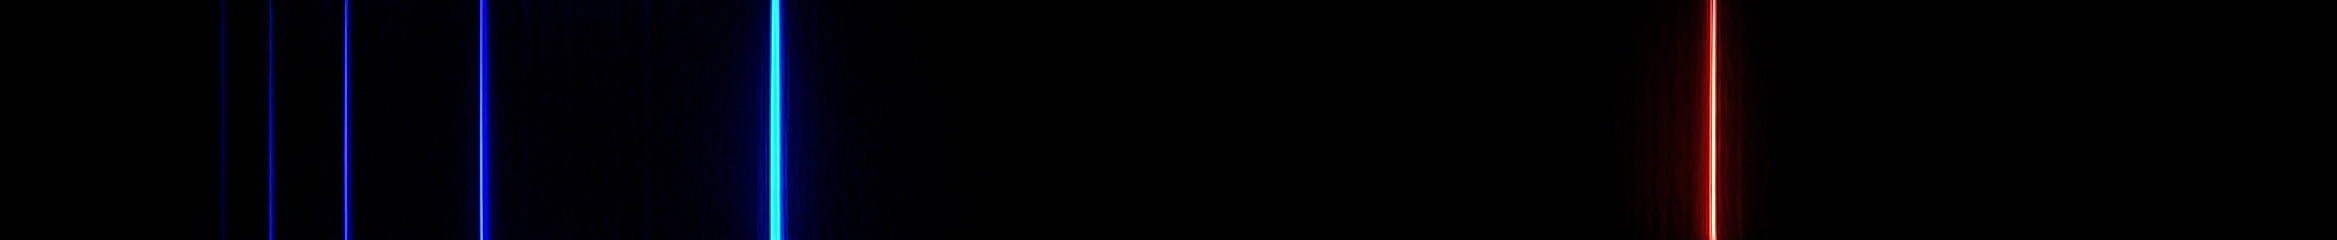
\includegraphics[width = .6\columnwidth]{../vortrag/pictures/wasserstoffSpektrum.jpg}
	\caption{Wasserstoffspektrum} %TODO \cite{link im owncloud ordner}}
	\label{atomuhr:wasserstoffspektrum}
\end{figure}

Auf der Abbildung \ref{atomuhr:wasserstoffspektrum} sieht man das Frequenzspektrum der sogenannte Balmer-Serie des Wasserstoffs, welche zufälligerweise im sichtbaren Bereich ist. Der rote Strich ganz rechts stellt die $H\alpha$-Linie dar. Die nächste links $H\beta$ und so weiter.


\subsection{Feinstruktur"ubergang}
Damit jedoch ein solcher "Ubergang elektrisch verarbeitet werden kann, muss es einen Effekt geben, bei welchem das Photon mit einer Frequenz im Gigahertz Bereich ausgesendet wird. 
Der Feinstruktur"ubergang ist ein erster Schritt in diese Richtung. 

Als das Wasserstoffspektrum genauer untersuchte wurde, bemerkte man, dass die Spektrallinien nicht atomar sind. Wenn man beispielsweise die $H\alpha$ Spektrallinie besser auflöst, so entdeckt man, dass diese eine Linie aus zwei besteht, welche sehr nahe aneinander liegen. 

\begin{figure}[h!]
	\centering
	%TODO im militär ist uploaden teuer, kopiere es dann in den richtigen Ordner, wenn ich zu Hause bin.
	
\includegraphics[width = .6\columnwidth]{../vortrag/pictures/fine_structure_hydrogen.png}
	\caption{$H\alpha$-Linie stark vergr"ossert, erkennbare Doppellinie} %TODO \cite{link im owncloud ordner}}
\end{figure}

Bis jetzt wurde nur mit der zeitunabhängigen Schr"odingergleichung gearbeitet.
Als erste N"aherung ist dies sicherlich nicht schlecht.
In der Realit"at spielt jedoch Zeitabh"angigkeit ein wichtiger Faktor. 
Mithilfe der St"orungstheorie ist es m"oglich, dieses Verhalten anzun"ahern.

\begin{itemize}
	\item[]  $H = \textcolor{red}{H_0}+ \textcolor{blue}{W_{SB}} + 
		\textcolor{green}{W_M} + \textcolor{violet}{W_D} $
	\item[]  $H$: relativistischer Hamiltonoperator
	\item[]  \textcolor{red}{$H_0$}: nicht relativistischer Hamiltonoperator
	\item[]  \textcolor{blue}{$W_{SB}$}: Spin Bahn Kopplung
	\item[]  \textcolor{green}{$W_M$}: Korrektur kin. Energie
	\item[]  \textcolor{violet}{$W_D$}: Korrektur pot. Energie
	
\end{itemize}
		
Auf die Korrekturfaktoren $W_M$ und $W_D$ wird hier nicht n"aher eingegangen, da diese nur zu geringf"ugigen Korrekturen f"uhrt und nicht f"ur die Doppellinie verantwortlich ist.

Der nicht relativistische Hamiltonoperator beschreibt das Bohrsche  Atommodell, welches bereits bekannt ist.

Bei der Spin Bahn Kopplung geht es um die reine Betrachtung des Elektrons. 
Dieses dreht sich in einer Kreisf"ormigen Bahn. 
Da das Elektron eine Ladung besitzt, entsteht ein magnetisches Feld. 
Dieses Feld wechselwirkt nun mit dem magnetischen Spin, den das Elektron auch noch besitzt. 
Da das Elektron entweder Spin +1/2 oder -1/2 hat, entstehen geringf"ugig unterschiedliche Frequenzen bei einem Quantensprung in das jeweilige Energielevel.

\begin{figure}
	\centering
	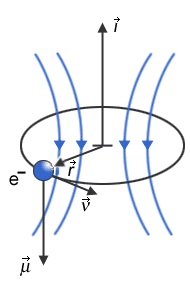
\includegraphics[width=.2\columnwidth]{../vortrag/pictures/feinstrukturelektron.jpg}
	\caption{Spin Bahn Kopplung} %TODO \cite{link im owncloud ordner}}
	\label{atomuhr:spinbahn}
\end{figure}

\subsubsection{Notation Termsymbol}
Jedes Atom hat nun verschiedene Entartungsgrade, in denen sich Elektronen befinden. Zus"atzlich ist die Annahme, dass das Elektron um das Atom kreist falsch. Die Elektronen befinden sich in einem bestimmten Sektor, welchem ein gewisser Bahndrehimpuls zugewiesen ist. 
Abbildung \ref{}
\begin{figure}
	\centering
	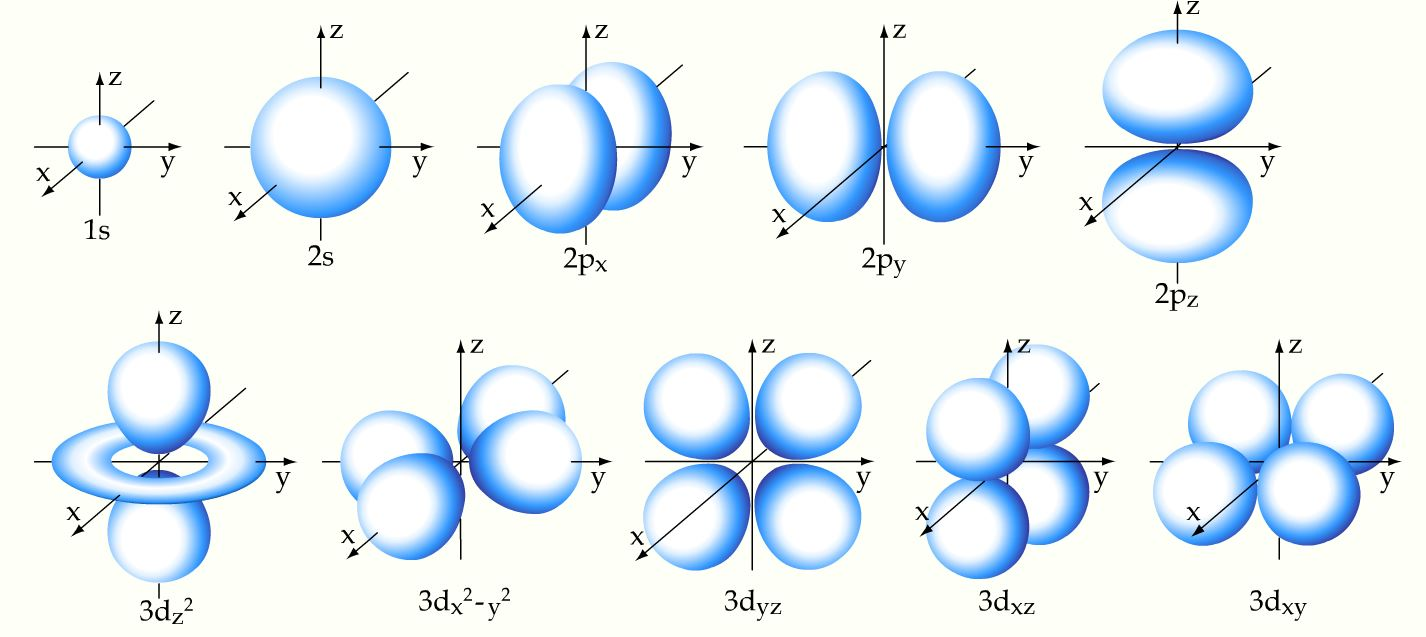
\includegraphics[width = 0.8\columnwidth]{../vortrag/pictures/orbitale.JPG}
	\caption{elektrische Bahndrehimpulse} %TODO \cite{link im owncloud ordner}}
	\label{atomuhr:bahndrehimpuls}
\end{figure}
Ausserdem hat das Elektron zwei verschiedene Spinzust"ande in dem es sich befinden kann. Der Aufenthaltsort eines Elektrons ist ein wenig komplizierter als noch beim Bohrschen Atommodell.
Dazu wurde die Termsymbol Notation entwickelt, welche den Zustand des Elektrons genau beschreibt. 
Diese wird nachfolgend kurz erkl"art.

\begin{equation}
	\text{Termsymbol:} \quad ^NL _J
\end{equation}

wobei

\begin{equation}
	J = L + S
\end{equation}

$N:$ Entartungsgrad

$L:$ elektrische Bahndrehimpuls

$J:$ Gesamtdrehimpuls

$S:$ Spin elektron

Dem elektrischen Bahndrehimpuls sind dabei den Zeichen folgende Zahlen zugewiesen.

\begin{table}
	\centering	
	\begin{tabular}{llll}
		s & p & d & f \\
		1 & 2 & 3 & 4 \\
	\end{tabular}
	\caption{elektrische Bahndrehimpulse}
	\label{atomuhr:drehimpulsnotation}
\end{table}

Mit diesem Wissen l"asst sich nun ein Feinstruktur"ubergang ausrechnen. 
\begin{center}
		"Ubergang: $^2P_{3/2} \rightarrow ^2P_{1/2}: \lambda = 2.76cm$
		
		$\nu_1 = \dfrac{c}{\lambda_1} = 10,9 GHz $
\end{center}

Das ausgesendete Photon befindet sich bei diesen Feinstruktur"uberg"angen in einem Bereich, in dem sie schon eher genutzt werden k"onnte. F"ur Atomuhren wird jedoch der  Hyperfeinstruktur"ubergang genutzt. 

\subsection{Hyperfeinstruktur"ubergang}
Der Feinstruktur"ubergang wurde entdeckt, als das Bohrsche Modell experimentell genauer untersucht wurde. "Ahnlich ergeht es dem Hyperfeinstruktur"ubergang. Als das Spektrum des Feinstruktur"ubergang besser aufgel"ost werden konnte, ist aufgefallen, das es noch einen Effekt gibt, welcher zu einer Aufspaltung eines Energielevels beim Feinstruktur"ubergang f"uhrt. Dieser wurde Hyperfeinstruktur"ubergang genannt und wird hier nun erkl"art.

Dieser Struktur"ubergang kann mithilfe der Wechselwirkung zwischen Elektron und Kern erkl"art werden. Der Kern besitzt einen gewissen Kernspin. Der magnetische Spin des Elektrons kann nun parallel oder antiparallel zum Kern sein. Was zu unterschiedlichen Energieniveaus f"uhrt. 

Beim Wasserstoff, welches im Grundzustand besetzt ist, führt das zu einer Wellenl"ange von $\lambda = 21\;cm$, was einer Frequenz von $\nu = 1.42\;GHz $ entspricht. Das ist eine Frequenz, welche sich sehr gut mit elektronischen Ger"aten verarbeiten l"asst. 

\subsection{Alkalimetalle}
Gleich wie Wasserstoff geh"ort auch Rubidium und C"asium zu den Alkalimetallen. speziell an dieser Gruppe von Elementen ist, dass sie nur ein freies Elektron in der letzten besetzten Schale haben. 

Da alle Atome Edelgaskonfiguration anstreben, wollen die Alkalimetalle dieses freie Elekron m"oglichst abgeben und sind dadurch relativ Reaktionsfreudig. 
Die abgeschlossenen Schalen sind elektrisch gesehen neutral. 
Weshalb die Alkalimetalle mutmasslich f"ur Atomuhren gebraucht wird. 
Das Frequenzspektrum ist einfacher zu verstehen als bei anderen Atomgruppen mit mehreren Valenzelektronen.

Rubidium hat einen Hyperfrequenz"ubergang von $\nu = 6.834\;GHz$. Die h"ohere frequenz l"asst sich damit erkl"aren, dass sich das Valenzelektron weiter weg vom Kern befindet als beim Wasserstoffatom. Die Kraft auf die Wechselwirkung ist somit kleiner. 

\section{Technische Betrachtung}

\subsection{Rechnung}

\section{Ausblick}

\subsection{SI-Basiseinheiten}
\label{sec:si-basiseinheiten}
Neben den direkt praktischen Einfl"usse einer genauen Zeitmessung, hat
eine genaue Sekundendefinition 

\section{Zusammenfassung}

\printbibliography[heading=subbibliography]
\end{refsection}

